\chapter{Introduction}
\section{Background}
As mobile devices continue their rapid run toward global adoption, mobile applications are extensively used in almost every aspect of our daily life. According to new data from Gartner \cite{gartner}, by 2017, mobile applications will be downloaded more than 268 billion times, generating revenue of more than \$77 billion and making applications one of the most popular computing tools for users across the globe. Together with the emergence of new applications, the rapid growth of mobile devices in both computing power and popularity leads to valuable renovations in many traditional mobile applications as well. For example, taking a quick look at the messaging application we can see a number of improvements (Figure \ref{fig:messaging_application}). Messaging applications today are capable of sending not only plain text messages but also images, videos, and other types of files. Furthermore, we can send messages to any place in the world via the Internet instead of relying on the local telephone companies. Regarding the user interface, in the past we could only read one message at a time but nowadays we can see the whole conversation conveniently thanks to the large and stunning display of smart phones. Not only are messaging applications improved, looking at the calling or note taking features of phones, we can see many enhancements as well.

\begin{figure}[!h]
\begin{centering}
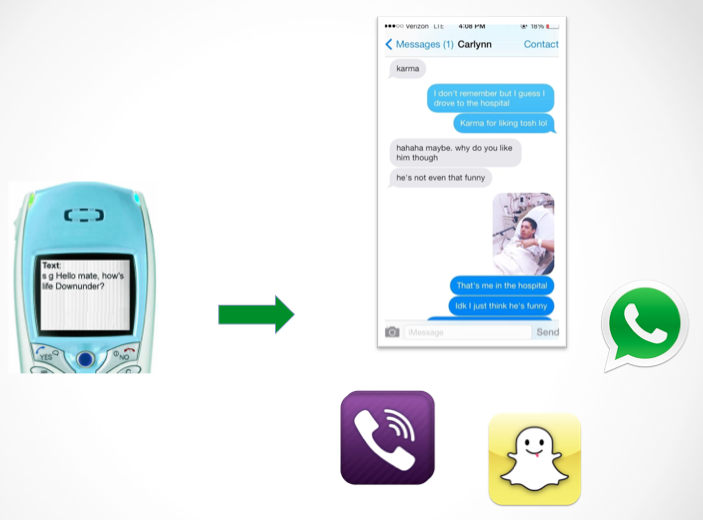
\includegraphics[scale=0.5]{pics/messaging_application}
\caption{Text Messaging Application Evolution}\label{fig:messaging_application}
\end{centering}
\end{figure}

However, there is one application that has not received much attention in the evolution of mobile phones: the Contacts application. People seem to ignore it although it has many potentials. In the past, the Contacts application was the site of initiating a few types of communications namely voice calls, text messages, and emails. Nowadays, with the emergence of new communication channels such as instant messaging \cite{Snapchat, Whatsapp}, Voice over IP \cite{Skype, Viber}, and social networks \cite{Facebook, Linkedin} the Contacts application can play an important role in creating a unified communication management interface. For example, instant messaging applications like Whatsapp \cite{Whatsapp} and Snapchat \cite{Snapchat} have been using the contacts of the devices as the identities for their users in order to eliminate the friends discovering and adding phases of normal chat applications. Some Voice over IP application such as Fring \cite{Fring} and Viber \cite{Viber} use this approach as well. Furthermore, in some modern mobile operating systems like Android \cite{Android}, when users select a contact on their devices they can choose to make a traditional voice call/text message or to use Voice over IP/instant messaging applications. Regarding social networks, we can link multiple social network profiles from Facebook \cite{Facebook}, LinkedIn \cite{Linkedin} to a phone contact via the similarities in email address and phone number. Beside all the new communication channels, voice calls and emails still act as the dominant communications in the business world since they are more formal. Therefore, the Contacts application is the central place for managing and widening people's connections.

\section{Problem Definition}

Regardless of playing a key role in users' connections, Contacts applications today have not changed much from their original form. All popular Contacts applications nowadays are merely ordered collections of contacts. As we can see from Figure \ref{fig:contactios} and Figure \ref{fig:contactandroid}, the contact profiles are a little more informative with the additions of profile pictures and some pre-defined fields, and yet, these additions are still limited. There are some big issues users still have to deal with their contacts which has not been solved:

\begin{enumerate}
    \item \textbf{Finding the right contact with some particular pieces of information}: T. Nguyen et. al \cite{tagging} through their study show that the majority of participants sometimes do not know who to call with a piece of information. The problem becomes more severe when it comes to looking up business or service contact information. They are the kind of long-term interaction which are infrequent but long-lasting contacts. The survey reveals that many people do not remember the name they use when creating the contact, hence they often have to browse the entire contacts list to find the number.
    \item \textbf{Recalling and retaining miscellaneous information of a contact}: When we have hundreds of contacts, remembering who they are and how we met them becomes an extremely difficult task especially for the contacts who we met quickly for business purposes. Whittaker et. al. \cite{Whittaker2002} emphasis that maintaining knowledge of the contacts is a critical problem. People are being exposed to an unmanageable number of contacts. Consequently, according to the researchers, users must decide: which of these contacts are valuable enough to maintain information about and what kinds of information to retain about the chosen contacts. Furthermore, recording the information is usually laborious and boring.
    \item \textbf{No support for establishing relationships between contacts}: If we connect the contacts inside one's Contacts application with each other, they will form a network. This network is remarkably similar to a social network like LinkedIn or Facebook. For instance, the profiles in both networks consist of basic information about real people and these profiles can be connected based on their real world relationships. Actually, according to Boyd and Ellison's definition \cite{boyd2010social}, the contact network satisfies all the criteria for a social network. However, this aspect has not been explored yet in modern Contacts applications. Since social networks have been developing incredibly and providing many benefits to its users, we believe not having the capability to establish relationships between the contacts in a Contacts application is a big omission. With the contact relationships, a Contacts application can answer a whole new class of user queries such as ``Find all colleagues of contact A'', ``Find the daughter of contact B''. This type of queries is currently impossible to accomplish in today Contacts application.
\end{enumerate}

\begin{figure}[!h]
\begin{centering}
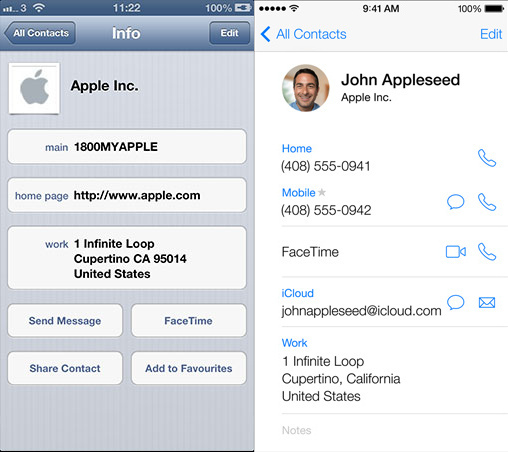
\includegraphics[scale=0.7]{pics/iphone}
\caption{Contacts Applications in iOS 6 and iOS 7}\label{fig:contactios}
\end{centering}
\end{figure}

% !!!
%Furthermore, Graphy can be integrated with other services such as users' mailboxes, text messages, call logs, etc. Therefore, it could automatically retrieve information related to a contact like email conversations, then provide these pieces of information when needed.
% Future work

\section{Research Goals}

In addressing the above mentioned issues, this research looks into developing a foundation model for contacts management applications which allows users to:

\begin{enumerate}[label=(\alph*)]
    \item find contacts by their miscellaneous information.
    \item efficiently retain knowledge of contacts. 
    \item establish relationships between contacts then traverse and explore the relationships with ease.
\end{enumerate}

In this regard, our research looks into creating Graphy - a prototype based on modern Contacts applications with improvements. Graphy fulfills the goal (a) by enabling users to create customized information for their contacts through a tags system. With the tags system, Graphy can act as a contacts ``search engine'' from which users can search for contacts with any particular characteristic. At the same time, the customized information tags also help users retaining various knowledge of their contacts (goal (b)). Besides customized information tags, Graphy automatically adds useful information like the location, the date, the event which the users are attending while they create a new contact to that contact's profile. These additional pieces of information create a context around the contact which assists users in recalling knowledge about it. Regarding goal (c), Graphy allows users to connect their contacts with each other to form an internal network which we call ``reversed social network''. We will explain details of this network and why we call it like that in Chapter 2. Furthermore, the emergence of Cloud Computing provides modern Contacts applications with the elegant capability of backup and sync data between multiple devices. Therefore, we want to ensure that our prototype is capable of exchanging data with the cloud using state-of-the-art technologies. Since all popular modern Contacts applications are closed source with proprietary software, we decide to develop our own communication and synchronization solution utilizing the trending RESTful communication technology. Our solution aim to make it easy for users to work offline through a local database while maintaining a central cloud database to backup and synchronize data to other devices when needed.

In short, the objectives of our prototype are as follows:

\begin{itemize}
    \item Operate like a modern Contacts application as well as provide additional improved features.
    \item Allow users to create customized information tags.
    \item Automatically add contextual information like the creation date and the creation location of a contact.
        \begin{itemize}
            \item The customized information tags and the contextual information should be searchable with rapid responses.
        \end{itemize}
    \item Allow users to establish relationships between contacts in a bi-directional manner.
        \begin{itemize}
            \item The relationships should be easy to traverse and explore.
        \end{itemize}
    \item Capable of backing up and synchronizing data to a server using RESTful communication.
\end{itemize}	

%The remainder of the thesis is organized as follows.

%we want our prototype to be able to 

%To tackle those problems, we have developed Graphy, a Contacts application which automatically adds useful information like the location, the date, the event which our users are attending while they create a new contact to that contact's profile. These additional pieces of information create a context around the contact which helps users recognize the contact. Besides auto-generated information Graphy enables users to create customized information for their contacts through a tags system. With the tags system, Graphy can act as a contacts search engine from which users can search for contacts with some specific features. Notably, all auto-generated information also remains as tags in the tags system thus being searchable as well. Concerning social networks, all modern Contacts applications have been providing integrations between their contacts and social networks' contacts from which users can merge these contacts together. Learning from that, Graphy not only utilizes this feature but also upgrades it to the next level. Beyond just integrating with outside social networks, Graphy introduces a novel internal network which connects contacts with each other. This internal network helps users explore relationships between their contacts - a task which is impossible for existing Contacts applications. 

% !!!
%Moreover, since social network visualizing is becoming more important \cite{freeman2000visualizing, Inmaps} Graphy provides its users with a graph connecting their contacts. Therefore, they can have a meaningful representation of all their phone book contacts. According to LinkedIn, with this representation users can better leverage their professional network to help seek advice, pass along opportunities, gather insights, and so forth \cite{linkedinblog}.

\begin{figure}[!h]
\begin{centering}
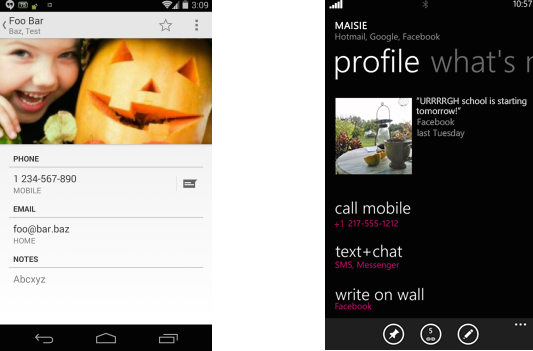
\includegraphics[scale=1.0]{pics/contacts}
\caption{Contacts Applications in Android 4.4, and Windows Phone 8.0}\label{fig:contactandroid}
\end{centering}
\end{figure}
